\chapter{Firmware inerciální jednotky}
Firmware hlavního \ac{MCU} byl vyvíjen pomocí volně dostupného \ac{IDE} poskytovaného výrobcem - \emph{STM32CubeIDE}. Jedná se o nástroj určený pro práci s jazyky C/C++, GCC kompilátorem založeném na Eclipse \cite{V2Tf5wsrbWcbQdoW}. Zároveň poskytuje grafické rozhraní pro konfiguraci a generování knihoven založených na \ac{HAL}, možnost použití \ac{RTOS} a ladící prostředí.

V této práci byly použity poskytované knihovny HAL a FreeRTOS pro ulehčení a urychlení vývoje firmwaru. Jejich použití často s sebou nese nevýhody, jako je například horší využití paměti, nebo výpočetního výkonu, z tohoto důvodu byl zvolen takový \ac{MCU}, aby měl dostatečné rezervy pro jejich použití.
\section{HAL}
Generování kódu \ac{HAL} v  STM32CubeIDE je možné pomocí grafického rozhraní, které poskytuje uživateli možnost nastavení jednotlivých pinů, periferií, komunikačních rozhraní a vnitřních hodin (obrázek \ref{fig:cubeConfig}). Vygenerované knihovny následně umožňují uživateli pracovat s \ac{MCU} s jistou mírou abstrakce, například není nutné znát a pracovat s názvy jednotlivých registrů. Typickým příkladem můžou být komunikační sběrnice (\ac{SPI}, \ac{I2C} \ldots), pro které jsou dostupné obslužné funkce na čtení a vysílání dat, jak v blokujícím režimu, tak i v neblokujícím (například pomocí \ac{DMA}). \cite{V2Tf5wsrbWcbQdoW}

Dále je možné pomocí stejného grafického rozhraní importovat rozšiřující softwarové balíčky, i když už se nejedná přímo o \ac{HAL}. V této práci byly použity \emph{FATFS} pro manipulaci se soubory na microSD kartě, \emph{FreeRTOS} jakožto jeden z dostupných \ac{RTOS} a \emph{USB\_DEVICE} pro práci s \ac{USB} rozhraním třídy \ac{MSC}.

\begin{figure}[h]
     \centering
     \begin{subfigure}[b]{0.4\textwidth}
         \centering
         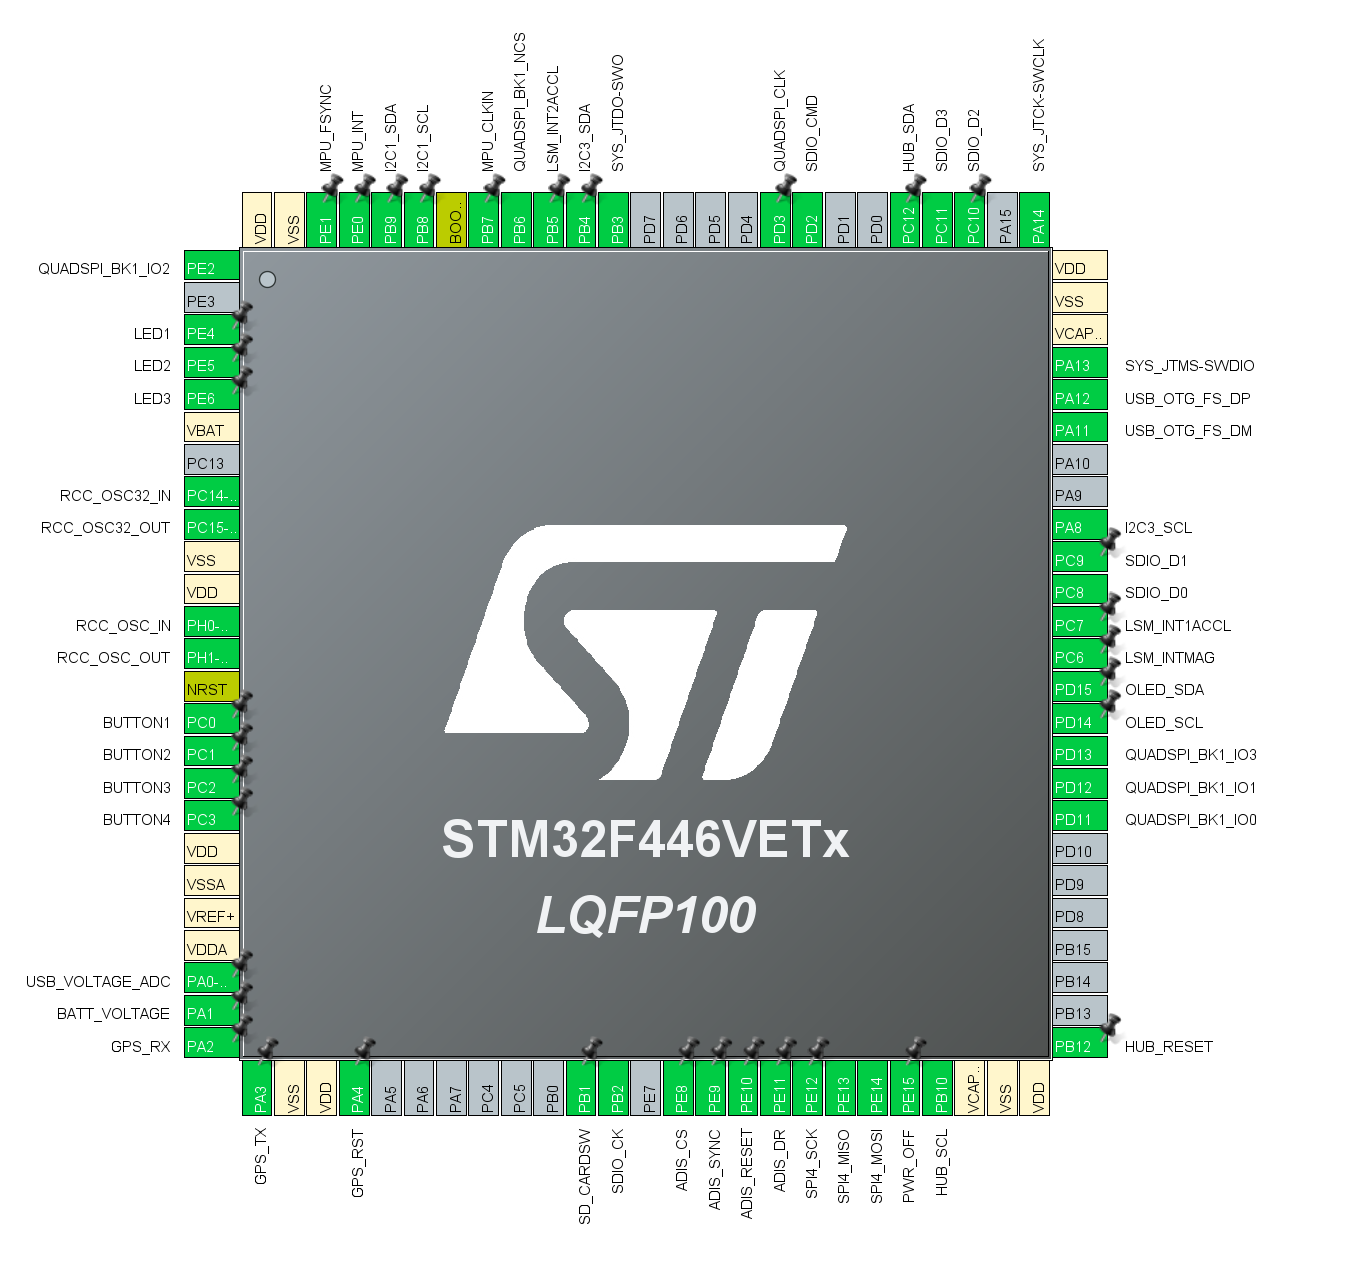
\includegraphics[width=\textwidth]{obrazky/cubePinout}
         \caption{Konfigurace pinů}
       
     \end{subfigure}
     \hfill
     \begin{subfigure}[b]{0.4\textwidth}
         \centering
         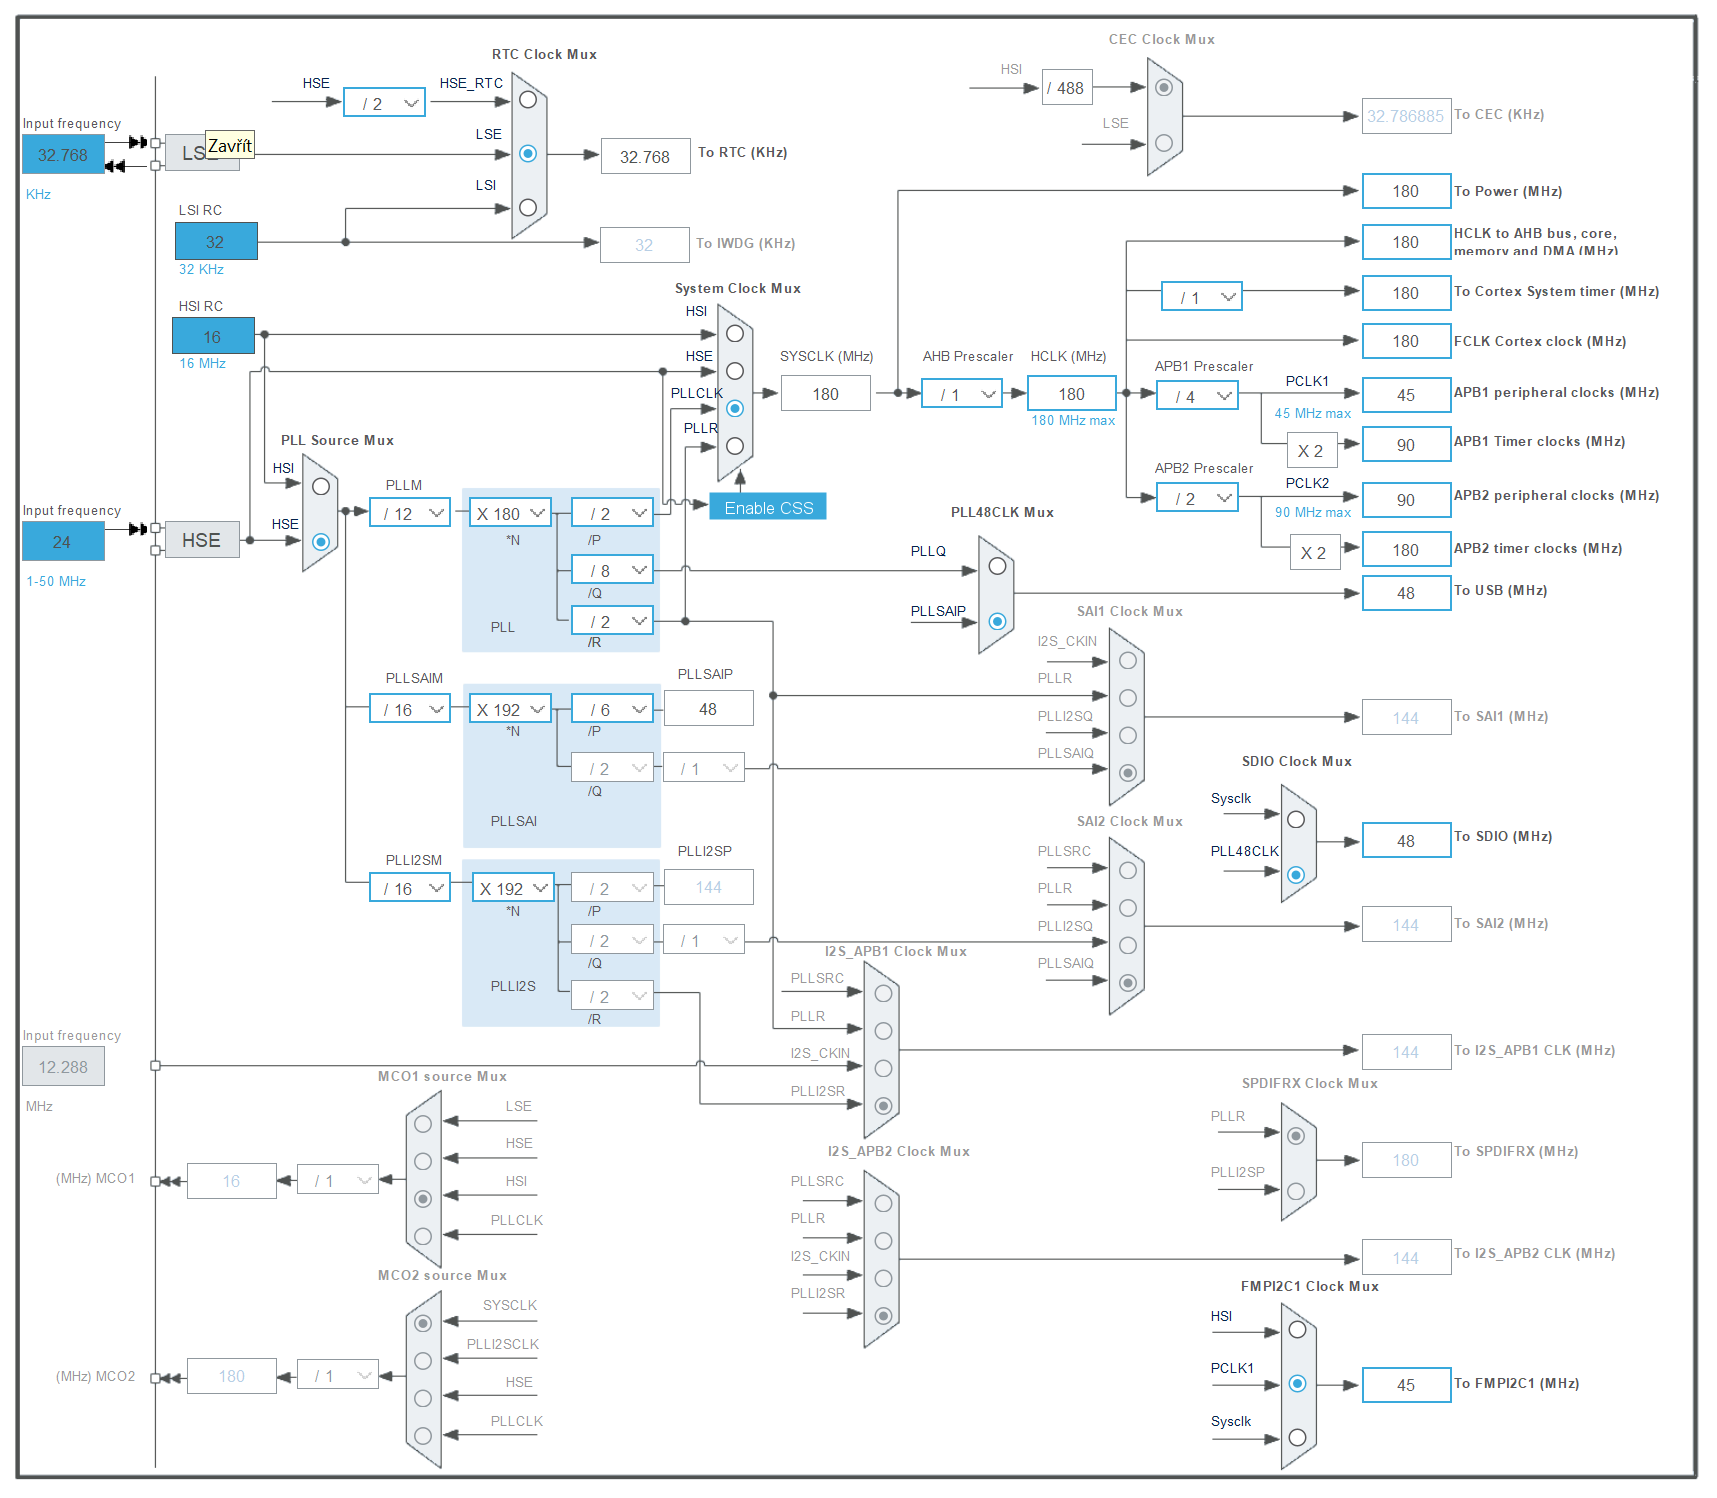
\includegraphics[width=\textwidth]{obrazky/cubeClock}
         \caption{Konfigurace hodin}
         
     \end{subfigure}
        \caption{Konfigurace MCU v STM32CubeIDE}
        \label{fig:cubeConfig}
\end{figure}

\section{FreeRTOS}
V této aplikaci je potřeba vyčítat, převádět a zapisovat data z několika různých senzorů které nemají přesně stejný hodinový signál, zároveň obsluhovat \ac{GUI} a provádět záznam dat. Pro potřeby synchronizace několika úloh, které nemají stejné periody, nebo například čekají na vstup od uživatele se hodí \ac{RTOS}.

Byla vybrána jedna z variant operačních systémů reálného času, a to FreeRTOS. Jedná se o jednoduchý open-source systém, který je hojně využíván ve vestavěných aplikacích. Umožňuje aplikaci virtuálně rozdělit na několik samostatných vláken (tzv. \emph{tasků}) s různými prioritami. Časování tasků je možné například pomocí neblokujících prodlev, nebo semaforů. FreeRTOS také plní funkci správy a alokace paměti. Předávání informací mezi jednotlivými tasky se provádí pomocí tzv. \emph{Queues}, které představují \ac{FIFO} zásobníky s nastavitelnou délkou fronty a velikostí jednotlivých dat. Díky tomu je možné se vyvarovat použití globálních proměnných. \cite{Zhu2011}

Práce s FreeRTOS je v STM32CubeIDE zjednodušená také díky poměrně dobré možnosti ladit aplikace pomocí již vestavěného RTOS-aware debuggeru, díky kterému můžeme například analyzovat využití paměti jednotlivých tasků, využití času, nebo kontrolovat stavy semaforů a velikost obsazených Queues. 

\section{Vývojové diagramy firmwaru}
Popsat chování a funkcionalitu firmwaru této aplikace dohromady by bylo poměrně nepřehledné. Proto budou jednotlivé funkce rozděleny do několika samostatných logických bloků, kde každý blok reprezentuje jeden task operačního systému.

Diagramy byly vytvořeny s úmyslem co nejlépe a nejjednodušeji reprezentovat chování jednotlivých tasků, proto i ty představují jistou míru abstrakce a neobsahují velké množství detailů, jako jsou různé prodlevy, obsluhy pinů, kontroly časovačů a podobně, aby byly diagramy lépe čitelné. Kompletní zdrojový kód je dostupný v elektronické příloze práce.

\subsection{KeepaliveTask}
\begin{figure}[h]
    \centering
    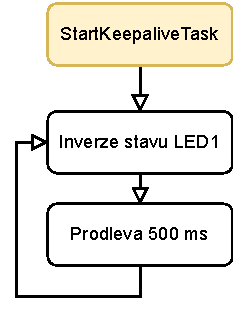
\includegraphics[width=0.22\textwidth]{obrazky/KeepaliveTask}
    \caption{Vývojový diagram KeepaliveTask}
\end{figure}
Jedná se o úlohu s nastavenou nejnižší prioritou. Slouží pouze pro ladicí účely a umožňuje jednoduchou a rychlou reprezentaci stavu systému pomocí blikající LED, zdali je spouštěn i task s nejnižší prioritou. V případě, že by LED přestala blikat, znamená to, že buď nějaký z vyšších tasků využívá výpočetní čas natolik, že se již nespustí úlohy s nižší prioritou, nebo došlo k chybě systému (například problémy přístupu do paměti)
\subsection{hubTask}
\begin{figure}[h]
    \centering
    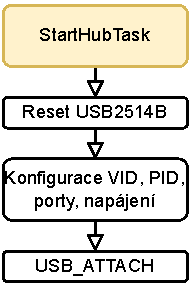
\includegraphics[width=0.18\textwidth]{obrazky/HubTask}
    \caption{Vývojový diagram HubTask}
\end{figure}
Tato úloha vykonává funkce pouze při zapnutí zařízení, a to konfiguraci a sepnutí vestavěného \ac{USB} rozbočovače. Do něj jsou nahrána konfigurační data pomocí sběrnice I2C, jako je například \ac{VID}, \ac{PID}, nastavení napájecího režimu a nastavení jednotlivých portů. U tohoto rozbočovače jsou zapnuty pouze využívané porty, aby byla snížena spotřeba zařízení. Následně jsou registry rozbočovače přepnuty do režimu pouze pro čtení a \ac{USB} rozhraní zapnuto. Při běhu zařízení již konfigurace zůstává stejná a task je neaktivní.
\subsection{powerTask}
V tomto tasku jsou periodicky měřena všechna analogová napětí pomocí \ac{ADC} procesoru, například napětí zdroje, USB portu, akumulátoru, ale i teplota procesoru. Tyto stavové veličiny jsou zobrazovány pomocí \ac{GUI}. Čtené hodnoty napětí akumulátoru jsou průměrovány pomocí pohyblivého exponenciálního filtru, který je možný zapsat pomocí rovnice \ref{eq:EMA}.

\begin{equation} \label{eq:EMA}
y[n]=\alpha \cdot x[n] + (1-\alpha)\cdot y[n-1]
\end{equation}

Kde $ x[n] $ je přečtená hodnota napětí, $ y[n] $ vyfiltrovaná hodnota napětí, $ y[n-1] $ výsledek vyfiltrované hodnoty napětí z předešlého cyklu a $ \alpha $ je nastavitelný koeficient odezvy filtru. Experimentálně bylo odzkoušeno, že vhodných výsledků filtrace šumu je možné dosáhnout s $ \alpha = 0,3$. Tento typ filtru byl zvolen zejména pro jeho jednoduchost a úsporné využití paměti.

V případě, že klesne napětí akumulátoru pod hranici 3,5 V je zařízení vypnuto překlopením S/R klopného obvodu, který je zmiňovaný v kapitole \ref{hardware} a tím je dosažena ochrana akumulátoru proti podvybití. Poté je možné zařízení znova zapnout pouze připojením do USB nabíječky.


\begin{figure}[h]
    \centering
    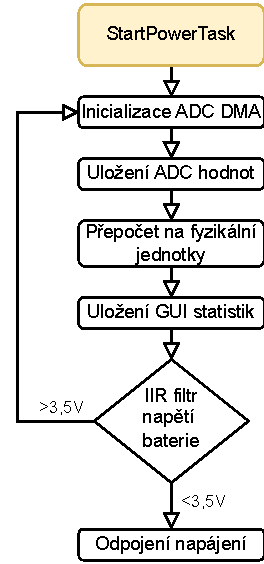
\includegraphics[width=0.25\textwidth]{obrazky/PowerTask}
    \caption{Vývojový diagram PowerTask}
\end{figure}
\subsection{gpsTask}
\begin{figure}[h]
    \centering
    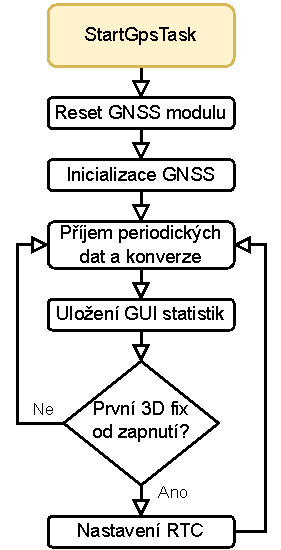
\includegraphics[width=0.25\textwidth]{obrazky/GpsTask}
    \caption{Vývojový diagram GpsTask}
\end{figure}
Tato úloha se stará o periodické zpracování příchozích dat z GNSS modulu pomocí \ac{UBX} zpráv. Tyto data jsou přijímány pomocí sběrnice \ac{UART} a je využito DMA přenosu, následně převedena do čitelné podoby (datum, čas, zeměpisná šířka, délka\ldots) pomocí knihovny GNSS parseru \cite{SimpleMethod2021}.

V této úloze je také kontrolováno kdy dojde k prvnímu přesnému určení polohy fixací na satelity a je aktualizován aktuální čas a datum do vnitřního \ac{RTC}.

\subsection{lsmTask} \label{lsmTask}
\begin{figure}[h]
    \centering
    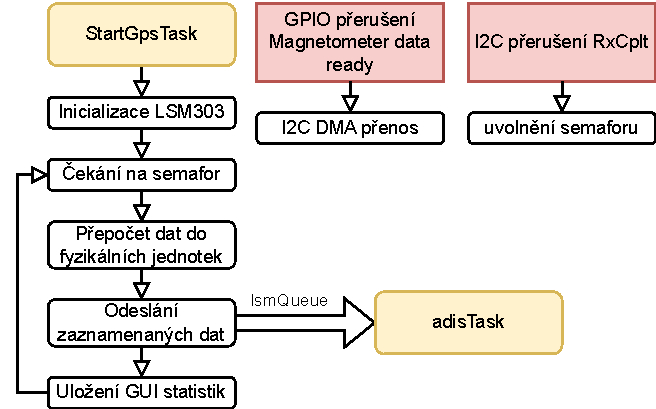
\includegraphics[width=0.6\textwidth]{obrazky/LsmTask}
    \caption{Vývojový diagram LsmTask}
\end{figure}
V tomto tasku jsou periodicky vyčítána data o magnetickém poli z elektronického kompasu LSM303. Ten je při zapnutí zresetován a následně inicializován rozsah, rozlišení a vzorkovací frekvence na 100 Hz. Po navzorkování dat magnetometr změní stav na svém pinu signalizujícím konec vzorkování. V ten okamžik je započat DMA přenos pomocí sběrnice I2C a jakmile jsou data vyčtena, převedou se do fyzikálních jednotek a odešlou se k záznamu. Využití DMA a přerušení data ready pinu senzoru nám umožňuje využívat plně neblokující kód, který má nízké využití výpočetního času MCU.

\subsection{mpuTask}
\begin{figure}[h]
    \centering
    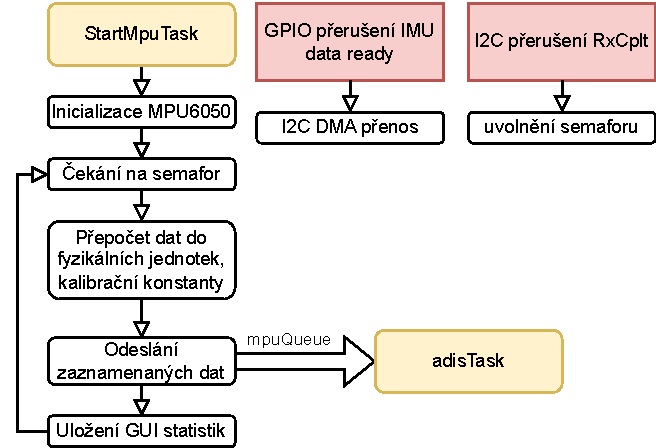
\includegraphics[width=0.6\textwidth]{obrazky/MpuTask}
    \caption{Vývojový diagram MpuTask}
\end{figure}
Tato úloha je velice obdobná předchozí z kapitoly \ref{lsmTask}. Zde jsou čtena a převáděna data z 6 osého IMU MPU6050 s frekvencí 400 Hz.

\subsection{adisTask}
\begin{figure}[h]
    \centering
    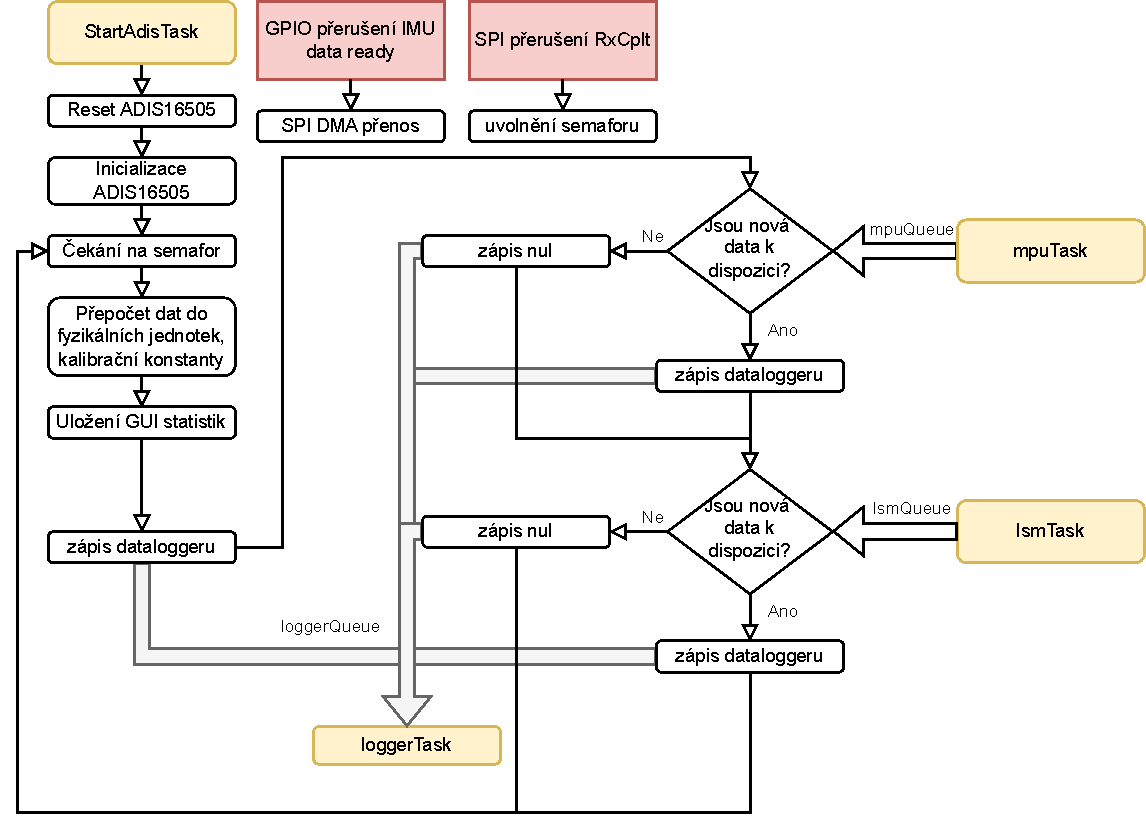
\includegraphics[width=0.95\textwidth]{obrazky/AdisTask}
    \caption{Vývojový diagram AdisTask}
\end{figure}
Tento task, obdobně jako předchozí, obstarává inicializaci, vyčítání a konverzi dat z 6 osého IMU ADIS16505 se vzorkovací frekvencí 400 Hz. Komunikace se senzorem probíhá přes sběrnici SPI a stejně jako u ostatních senzorů, je využíváno přerušení a DMA přenosů k vytvoření neblokujícího kódu. Vzhledem k vyššímu rozlišení senzoru v porovnání s ostatními je pro ukládání hodnot převedených do jednotek SI využíván datový typ \texttt{double} místo \texttt{float}.

Vzorkování dat z ADIS16505 zároveň slouží jako synchronizace k zarovnání řádků dat ve výsledném souboru naměřených dat, tedy v případě, že jsou dostupná nová data z LSM303, nebo MPU6050, jsou přidána do celkové záznamové datové struktury, v opačném případě jsou na jejich odpovídající místa zapsány nuly. V nejhorším možném případě, tedy že data z ostatních senzorů jsou vzorkována těsně po navzorkování dat z ADIS16505 je jejich zpoždění délka jedné periody celkové vzorkovací frekvence, tedy 2,5 ms.

\subsection{loggerTask}
\begin{figure}[h]
    \centering
    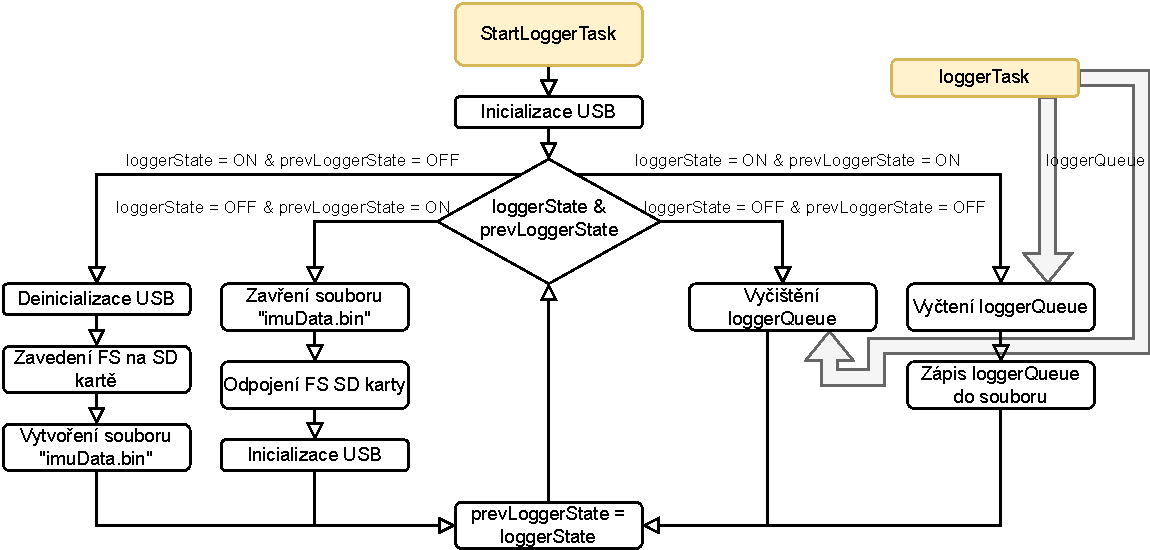
\includegraphics[width=0.99\textwidth]{obrazky/LoggerTask}
    \caption{Vývojový diagram LoggerTask}
\end{figure}
Tato úloha provádí samotné ukládání dat. Testováním bylo zjištěno, že při použití kvalitnějších microSD karet (v zařízení je použita \emph{SAMSUNG 64GB EVO PLUS}) nedochází k náhodným delším prodlevám při zápisu. Zároveň v porovnání s NOR FLASH pamětí poskytuje řádově větší úložiště, rychlejší zápis bloku dat, není potřeba mazat každý sektor paměti před zápisem a také je jednoduší implementace souborového systému. Z těchto důvodů bylo rozhodnuto využití SD karty k ukládání měřených dat.

Stavový automat v tomto tasku lze rozdělit do čtyř stavů: záznam dat, kdy jsou data průběžně ukládána, vypnutý záznam, kdy jsou data zahazována a začátek a konec záznamu, kdy dochází k inicializacím USB a souborových systémů. V průběhu záznamu je USB rozhraní vypnuté, aby nebylo možné zasahovat do souboru připojeným PC když je zrovna do něj zapisováno zařízením.

Samotný přenos naměřených dat do počítače je realizován přes USB třídy vysokokapacitního úložiště. Připojený PC při potřebě čtení dat spustí přerušení na přenos s konkrétní adresou. Jelikož je na microSD kartě implementován souborový systém FatFS, je v běžných operačních systémech reprezentován jako obyčejné externí úložiště.

\subsection{oledTask}
\begin{figure}[h]
    \centering
    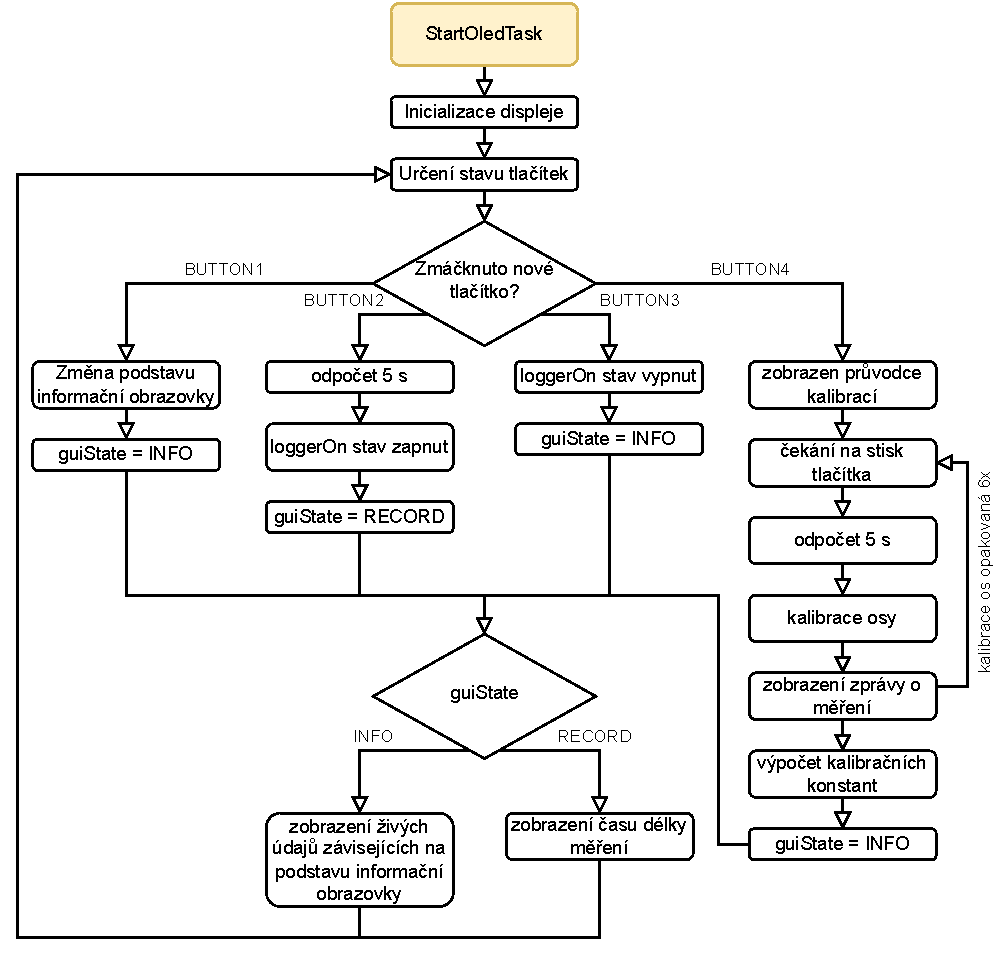
\includegraphics[width=0.8\textwidth]{obrazky/OledTask}
    \caption{Vývojový diagram OledTask}
\end{figure}
Tento task obstarává obsluhu uživatelského rozhraní pomocí grafického displeje a čtveřice tlačítek. Při každém cyklu
je porovnán předchozí a stávající stav tlačítek. Jestliže došlo k nějakému stisknutí, změní se náležitě zobrazované informace a chování zařízení. Displej komunikuje s \ac{MCU} přes sběrnici I2C a k ovládání byla použita knihovna řadiče SSD1306 \cite{Alekseev2024}. Funkce jednotlivých tlačítek jsou reprezentovány ikonami ohraničenými rámečkem na spodní straně displeje.

Stav zařízení by se dal zjednodušeně znázornit třemi možnými:
\begin{itemize}
\item Výchozí obrazovka stavových informací (obrázek \ref{fig:stateInfoGUI}) - pomocí ní je možné odečítat okamžité hodnoty veličin měřených senzory a zařízením. Při zapnutí je zobrazena výchozí domovská obrazovka, na které jsou přítomny provozní informace, jako je napětí akumulátoru, teplota procesoru, nebo čas uložený v RTC. Stisky tlačítka 1 (reprezentováno ikonou HOME na displeji) je možné měnit zobrazované informace na jednotlivé IMU, elektronický kompas a GNSS modul. Při změně obrazovky se také náležitě obmění levá spodní ikona reprezentující tlačítko 1. Všechny senzorové veličiny (lineární zrychlení, úhlová rychlost, velikost magnetické indukce) jsou již převedeny a zobrazeny v jednotkách soustavy SI.
\begin{figure}[h]
     \centering
     \begin{subfigure}[b]{0.29\textwidth}
         \centering
         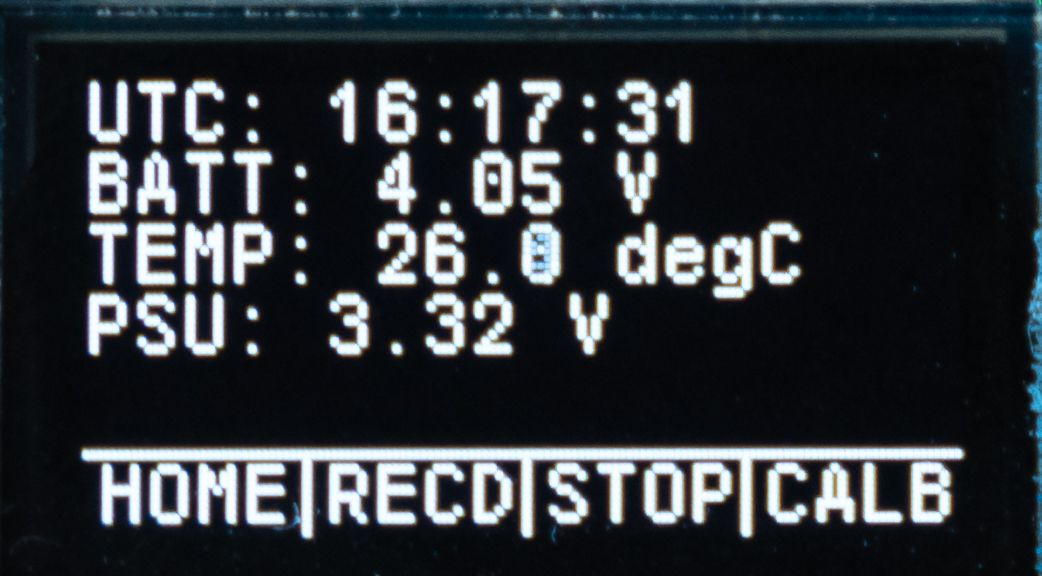
\includegraphics[width=\textwidth]{obrazky/menuHome2}
         \caption{Domovská obrazovka}
       
     \end{subfigure}
     \hfill
     \centering
     \begin{subfigure}[b]{0.29\textwidth}
         \centering
         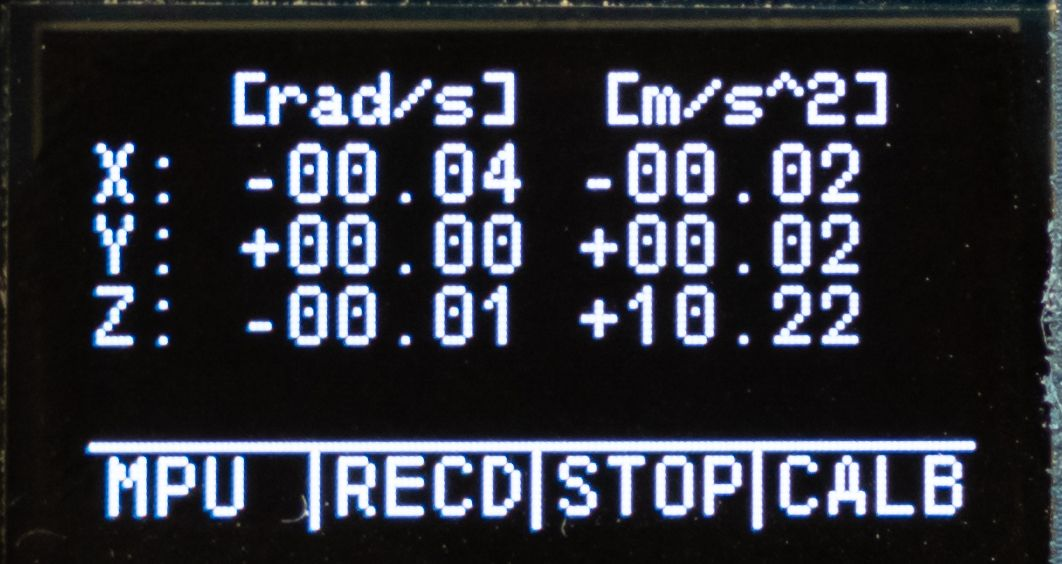
\includegraphics[width=\textwidth]{obrazky/menuMPU}
         \caption{Hodnoty z MPU6050}
         
     \end{subfigure}
     \hfill
     \centering
     \begin{subfigure}[b]{0.29\textwidth}
         \centering
         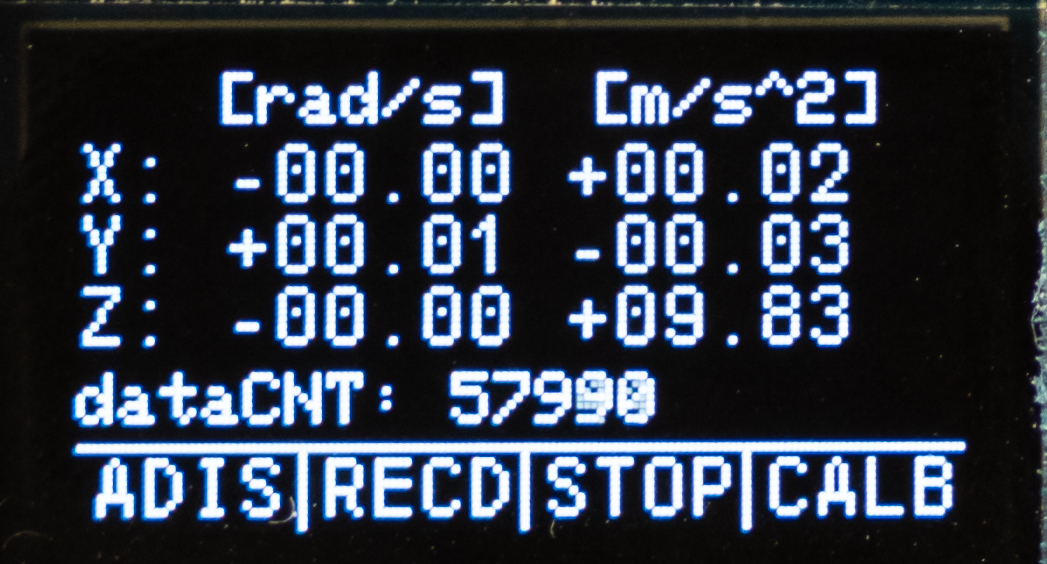
\includegraphics[width=\textwidth]{obrazky/menuADIS}
         \caption{Hodnoty z ADIS16505}
       
     \end{subfigure}
     \centering
     \begin{subfigure}[b]{0.29\textwidth}
         \centering
         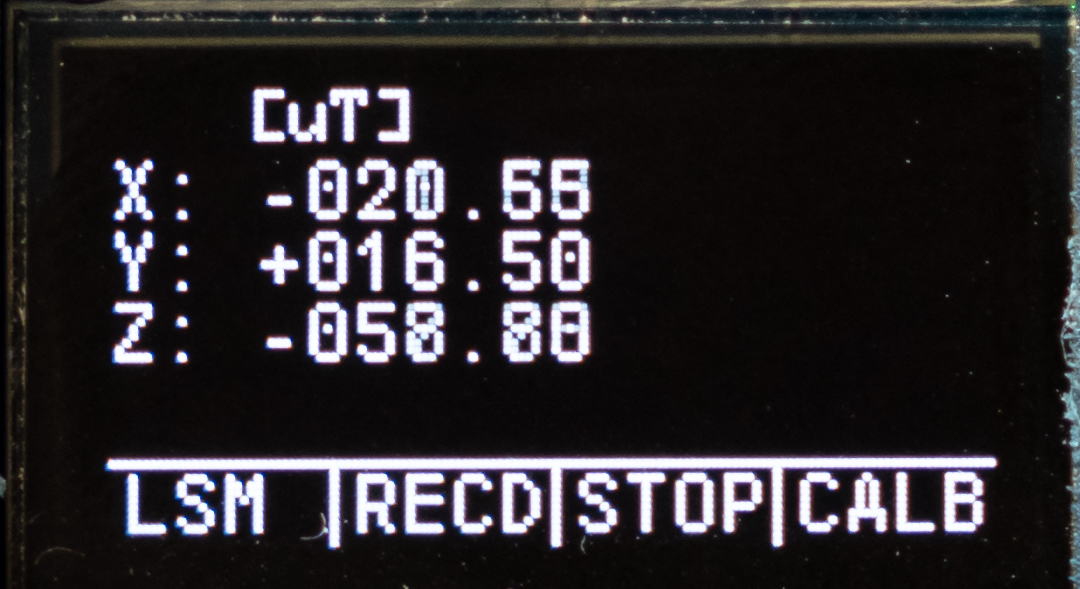
\includegraphics[width=\textwidth]{obrazky/menuLSM}
         \caption{Hodnoty z LSM303}
       
     \end{subfigure}
		\hfill
     \begin{subfigure}[b]{0.29\textwidth}
         \centering
         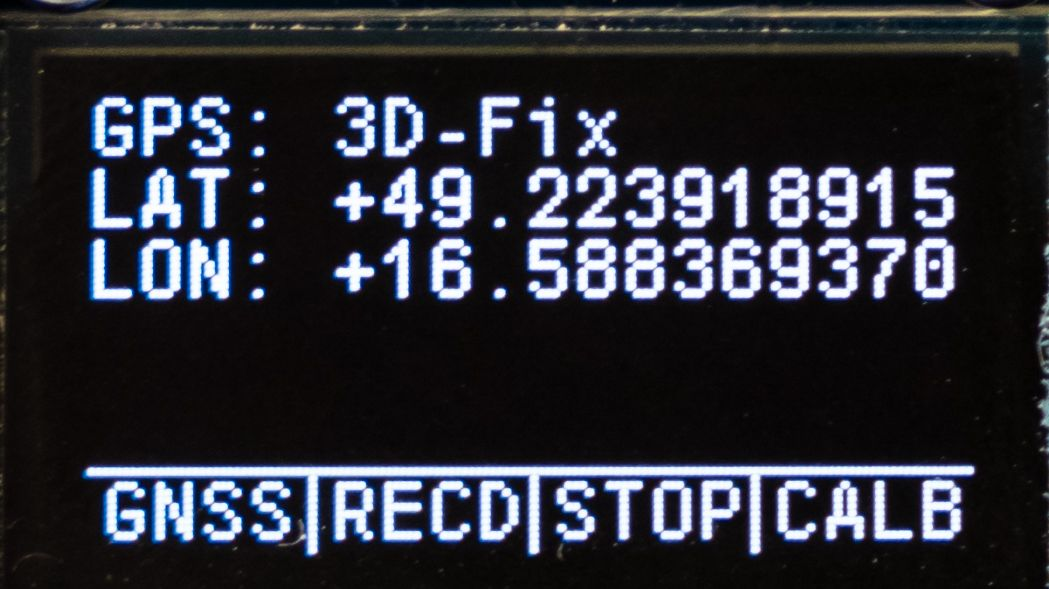
\includegraphics[width=\textwidth]{obrazky/menuGPS}
         \caption{Hodnoty z GNSS}
         
     \end{subfigure}

        \caption{GUI stavových informací jednotlivých senzorů}
        \label{fig:stateInfoGUI}
\end{figure}

\item Záznam dat (obrázek \ref{fig:recordGUI}) - Ten je možné aktivovat stiskem tlačítka 2, kterému náleží ikona RECD. Po jeho stisknutí je na displeji zobrazen pětisekundový odpočet, který slouží k tomu, aby uživatel umístil jednotku do nehybného stavu (i samotný zákmit ze stisku tlačítka může velice ovlivnit měření) a až poté je zapnut záznam dat. V průběhu záznamu je uživateli zobrazována délka zaznamenaných dat (v sekundách) a není nijak omezena. Záznam dat je poté možné přerušit stiskem tlačítka 3, kterému odpovídá ikona STOP.

\begin{figure}[h]
     \centering
     \begin{subfigure}[b]{0.29\textwidth}
         \centering
         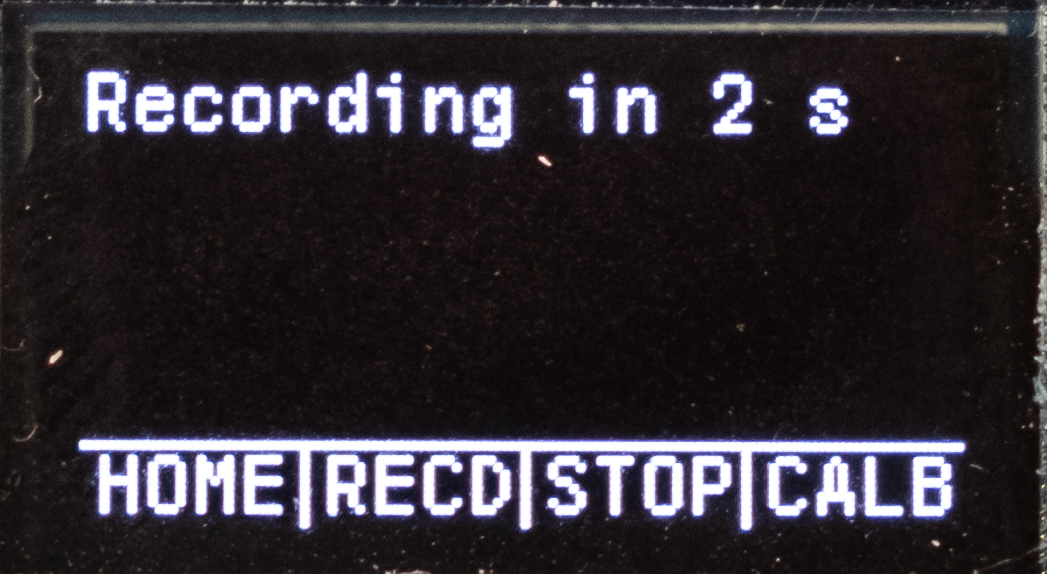
\includegraphics[width=\textwidth]{obrazky/menuREC1}
         \caption{Odpočet startu}     
     \end{subfigure}
     \hfill
     \centering
     \begin{subfigure}[b]{0.29\textwidth}
         \centering
         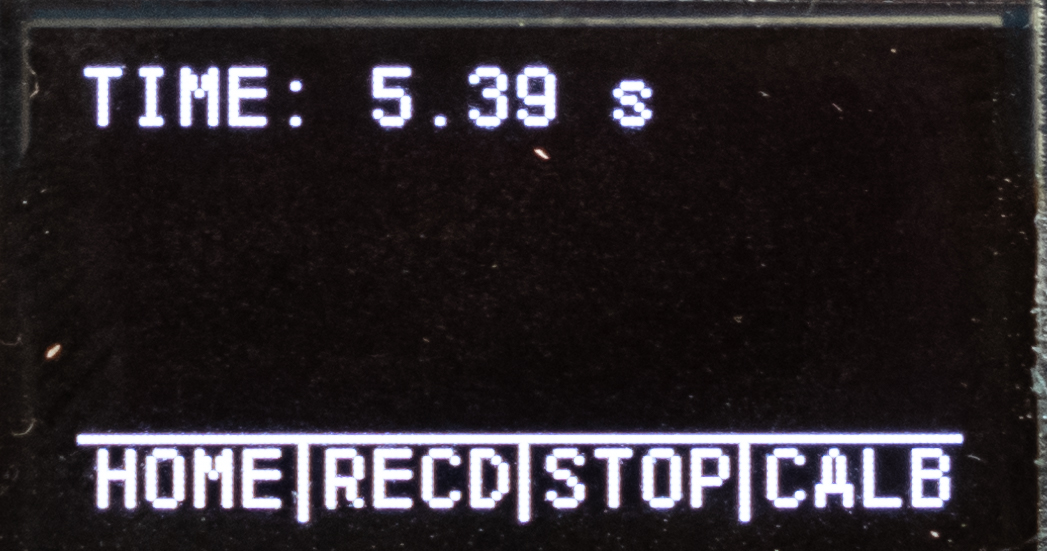
\includegraphics[width=\textwidth]{obrazky/menuREC2}
         \caption{Délka záznamu dat}   
     \end{subfigure}

        \caption{GUI záznamu dat}
        \label{fig:recordGUI}
\end{figure}

\item Kalibrace (obrázek \ref{fig:calibrationGUI})- toto menu slouží jako průvodce kalibrační procedurou. Aktivuje se stiskem tlačítka 4, kterému odpovídá ikona CALB. Následně je uživateli zobrazen dvoustránkový průvodce kalibrační procedurou, který popisuje jednotlivé kroky potřebné k úspěšnému provedení kalibrace. Poté je uživatel vyzván k umístění jednotky na jednu z 6 hran a po pětisekundovém odpočtu je změřeno 50 vzorků lineárního zrychlení a úhlové rychlosti z obou IMU a vypočítán jejich průměr. Tento postup se opakuje šestkrát s každou hranou zařízení. Následně jsou z měření vypočteny kalibrační konstanty pomocí algoritmu popsaným v kapitole \ref{calibrationALG}.
\end{itemize}
\begin{figure}[h]
     \centering
     \begin{subfigure}[b]{0.24\textwidth}
         \centering
         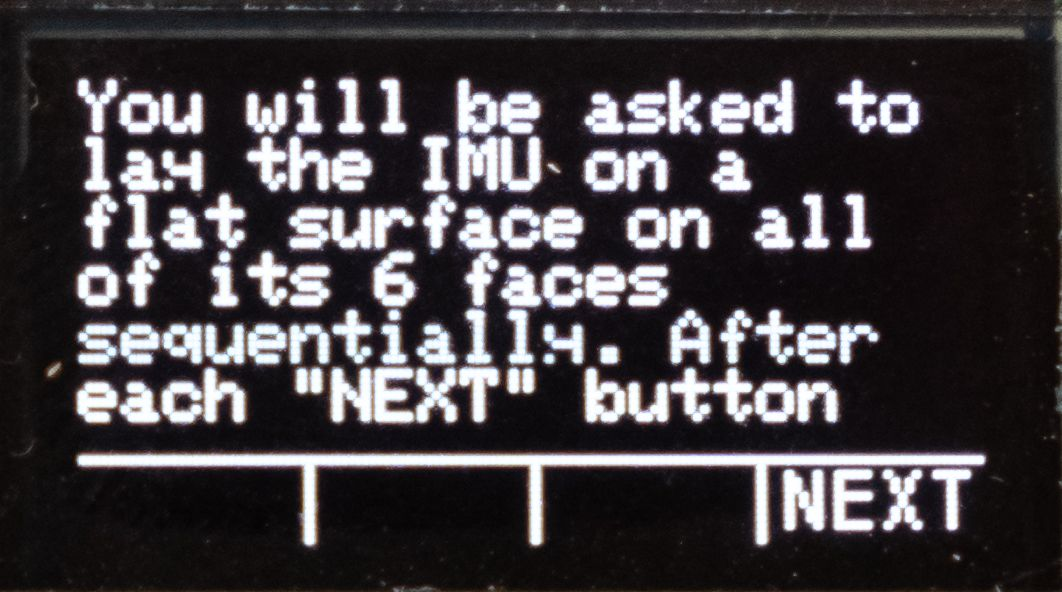
\includegraphics[width=\textwidth]{obrazky/menuCAL1}
         \caption{Průvodce 1}     
     \end{subfigure}
     \hfill
     \centering
     \begin{subfigure}[b]{0.24\textwidth}
         \centering
         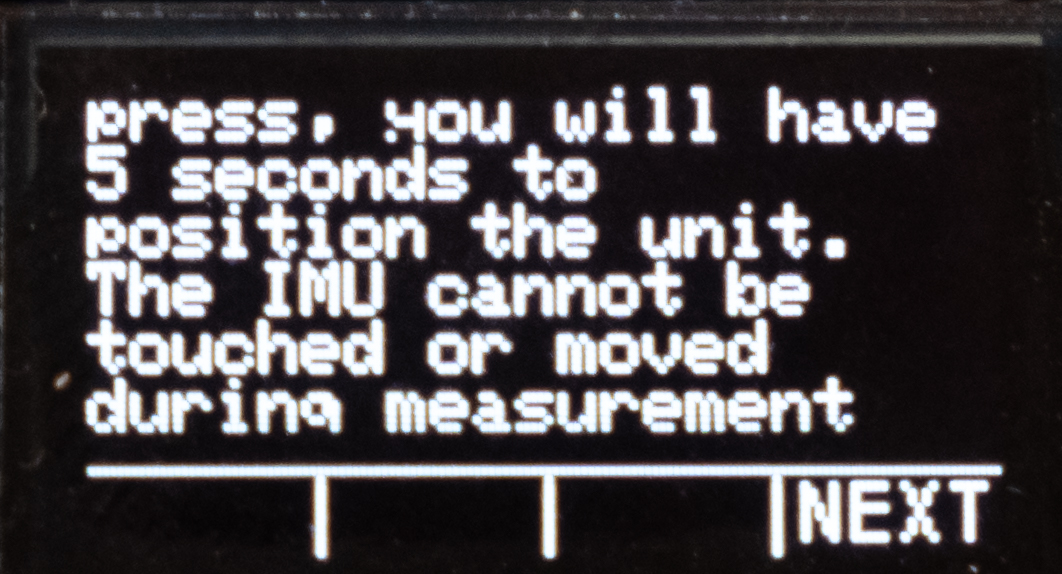
\includegraphics[width=\textwidth]{obrazky/menuCAL2}
         \caption{Průvodce 2}   
     \end{subfigure}
     \hfill
          \centering
     \begin{subfigure}[b]{0.24\textwidth}
         \centering
         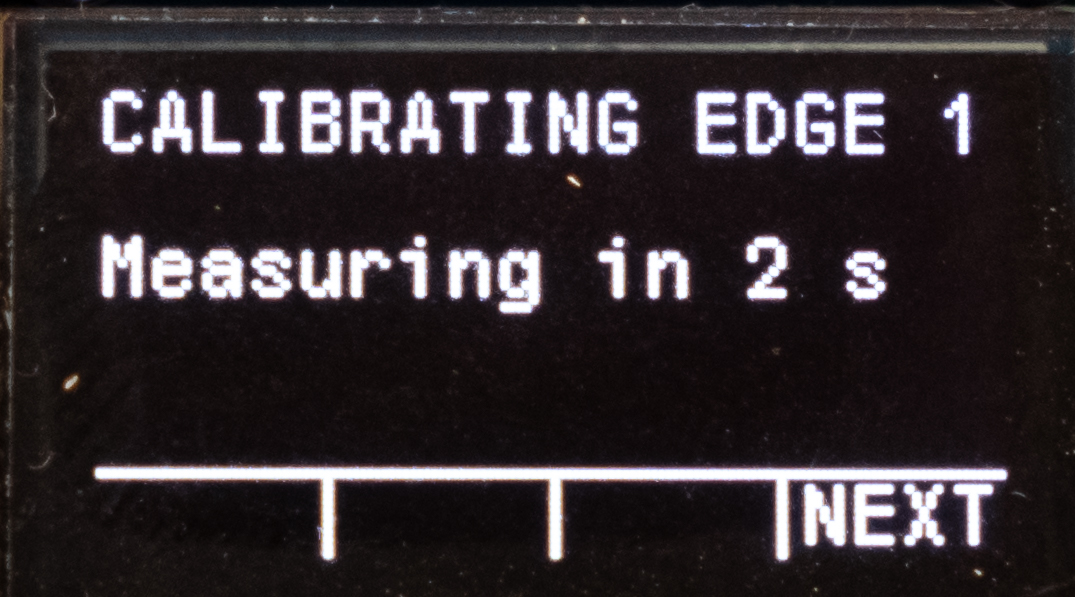
\includegraphics[width=\textwidth]{obrazky/menuCAL3}
         \caption{Odpočet měření}     
     \end{subfigure}
     \hfill
     \centering
     \begin{subfigure}[b]{0.24\textwidth}
         \centering
         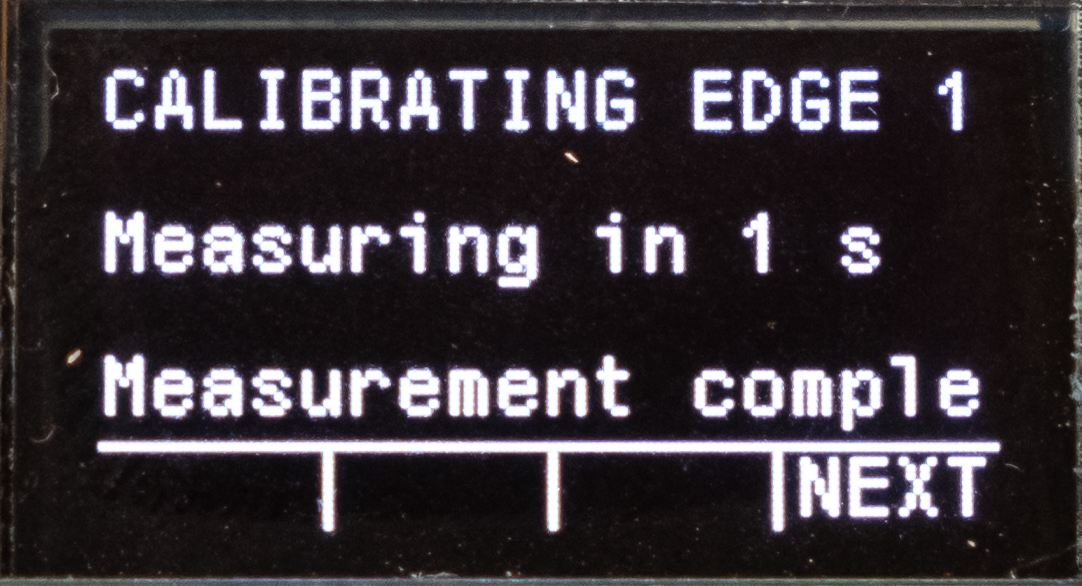
\includegraphics[width=\textwidth]{obrazky/menuCAL4}
         \caption{Hotový záznam}   
     \end{subfigure}

        \caption{GUI kalibrační procedury}
        \label{fig:calibrationGUI}
\end{figure}

\section{Kalibrace IMU} \label{calibrationALG}
Akcelerometry a gyroskopy jsou poměrně citlivé součástky. Přestože většina i těch levnějších IMU jsou v továrně výrobcem kalibrovány, jejich vlastnosti se můžou změnit například procesem pájení, změnou teploty, nebo mechanickým pnutím v desce plošných spojů. Drtivá většina popsaných kalibračních metod akcelerometrů se zaměřuje na korekci lineární křivkou, jedná se tedy o výpočet konstant k a q v rovnici $ y=k\cdot x + q $, kde $ x $ je měřená hodnota senzorem, $ k $ a $ q $ jsou kalibrační konstanty a $ y $ je výsledná veličina po kalibraci. Konstantu $ k $ můžeme označit jako gain a konstantu $ q $ jako offset. Většinou se dostupné metody kalibrací používají i pro kompenzaci odchylek natočení os senzorů vůči desce, nebo nějakému jinému referenčnímu prvku zařízení (například hrany krabice), které můžou vzniknout nepřesným pájením, nebo montáží. Tyto metody vyžadují buď nějaké přípravky, které nám umožní otáčet se zařízením o přesně definovaný úhel v pravoúhlých osách, nebo alespoň vyžadují přesné natáčení zařízení do poloh, kde dvě z os měří nulové zrychlení. \cite{eUM5mr8dMf0LyseX} \cite{6yeG6wAI1hTfmXJK}

V této práci ovšem není až tak důležité kompenzovat natočení os senzorů, jelikož je zařízení určené pro manipulaci v rukách, jde nám tedy pouze o výpočet konstant $ k $ a $ q $, aby bylo měřeno zrychlení správné velikosti. Výroba výše zmíněných mechanických přípravků, které by byly dostatečně přesné a opakovatelné by byla náročná a nesouvisející s povahou této práce. Díky tomu, že nepotřebujeme kompenzovat natočení os, můžeme vycházet z dostupných kalibračních procedur a implementovat jejich podstatu v upravené podobě:

Kalibrační procedura vychází ze znalosti velikosti tíhového zrychlení. Budeme-li mít akcelerometr nehybný, tak v jakékoliv jeho pozici by velikost vektoru zrychlení měla být rovna tíhovému zrychlení. To můžeme zapsat pomocí rovnice \ref{eq:sizeOfVect}.

\begin{equation} \label{eq:sizeOfVect}
\lvert\vec{a}\rvert=\sqrt{\lvert\vec{a_{x}}\rvert^{2}+\lvert\vec{a_{y}}\rvert^{2}+\lvert\vec{a_{z}}\rvert^{2}}=\lvert\vec{g}\rvert
\end{equation} 

Za velikosti zrychlení dosadíme měřené hodnoty akcelerometrem, korigované lineární křivkou. Dostaneme rovnici \ref{eq:sizeOfCalVector}.

\begin{equation} \label{eq:sizeOfCalVector}
\lvert\vec{g}\rvert=\sqrt{(k_{x}\cdot a_{x} + q_{x})^{2}+(k_{y}\cdot a_{y} + q_{y})^{2}+(k_{z}\cdot a_{z} + q_{z})^{2}}
\end{equation} 

Cílem je tedy určit konstanty k a q. K tomu je potřeba vyřešit nelineární rovnici o šesti neznámých. K řešení provedeme 6 měření a vytvoříme soustavu 6 nelineárních rovnic o 6 neznámých z rovnice \ref{eq:sizeOfCalVector}. Teoreticky nezáleží na natočení zařízení v průběhu 6 zmiňovaných měření, jelikož je počítána velikost vektoru zrychlení ze tří ortogonálních os senzoru, ovšem nejlepších výsledků dostaneme když natočíme zařízení na všechny z 6 stran krabičky zařízení (pravý bok, levý bok, spodní strana, horní strana, přední strana a zadní strana) jelikož v těchto případech budou měřena maxima a minima zrychlení pro všechny osy. Pokud bychom totiž provedli 6 měření v úplně stejné poloze zařízení, může se stát, že použitá numerická metoda řešení rovnic konverguje k řešení typu všechny gainy budou nulové a offset v jedné ose bude roven velikosti tíhového zrychlení. Toto řešení by bylo matematicky správné, ale nedávalo by smysl.

Jednou z možností, jak kalibraci provést by bylo tzv. "offline", tedy provést kalibrační měření a následně data přenést do počítače a kalibrační konstanty vypočítat například pomocí MATLABu. To by ovšem omezilo univerzálnost vyvíjeného zařízení, také by byla kalibrace poměrně složitá a nemotorná z pohledu uživatele. Jako pohodlnější řešení byla zvolena implementace metody nejmenších čtverců pomocí funkce \texttt{fsolve} ve spojení s \emph{MATLAB Coder}.

Nejdříve byla vytvořena následující funkce, která slouží k určení všech 6 kalibračních konstant akcelerometru. Tyto kalibrační konstanty jsou uložené do výstupního vektoru \texttt{x}. Vstupními argumenty je matice \texttt{accel(6,3)}, která obsahuje naměřené zrychlení a \texttt{gravityScalar}, což je velikost tíhového zrychlení.

\begin{lstlisting}[
frame=single,
numbers=left,
style=Matlab-Pyglike,
 basicstyle=\fontsize{9}{10}\selectfont\ttfamily]
function [x,fval] = AccelCalSolver(accel, gravityScalar) %#codegen
% The directive %#codegen indicates that the function
% is intended for code generation
arguments
    accel (6,3) double
    gravityScalar   (1,1) double
end


fun = @(x)gravityFun(x, accel, gravityScalar);%gravity function handler
x0 = [1 0 1 0 1 0]; % Initial point - gain=1, offset=0
options = optimoptions('fsolve','Algorithm','levenberg-marquardt','Display','off');
[x,fval] = fsolve(fun, x0, options);

end
\end{lstlisting}

Kořeny rovnice jsou vyřešeny metodou nejmenších čtverců s výchozími body gain = 1 a offset = 0. Samotný tvar matice je definován v samostatném souboru a obsahuje šest rovnic \ref{eq:sizeOfCalVector} v upraveném tvaru:
\begin{lstlisting}[
frame=single,
numbers=left,
style=Matlab-Pyglike,
 basicstyle=\fontsize{9}{10}\selectfont\ttfamily]
function F = gravityFun(x, accel, gravityScalar)
F = zeros(6,1); % Allocate return array


F(1) = (accel(1,1)*x(1) + x(2))^2 + (accel(1,2)*x(3) + x(4))^2 + (accel(1,3)*x(5) + x(6))^2 - gravityScalar^2;
F(2) = (accel(2,1)*x(1) + x(2))^2 + (accel(2,2)*x(3) + x(4))^2 + (accel(2,3)*x(5) + x(6))^2 - gravityScalar^2;
F(3) = (accel(3,1)*x(1) + x(2))^2 + (accel(3,2)*x(3) + x(4))^2 + (accel(3,3)*x(5) + x(6))^2 - gravityScalar^2;
F(4) = (accel(4,1)*x(1) + x(2))^2 + (accel(4,2)*x(3) + x(4))^2 + (accel(4,3)*x(5) + x(6))^2 - gravityScalar^2;
F(5) = (accel(5,1)*x(1) + x(2))^2 + (accel(5,2)*x(3) + x(4))^2 + (accel(5,3)*x(5) + x(6))^2 - gravityScalar^2;
F(6) = (accel(6,1)*x(1) + x(2))^2 + (accel(6,2)*x(3) + x(4))^2 + (accel(6,3)*x(5) + x(6))^2 - gravityScalar^2;

end
\end{lstlisting}

Také byla vytvořena testovací funkce na její ověření. Všechny zdrojové kódy jsou také dostupné v elektronické příloze. MATLAB umožňuje vytvořit zdrojový kód v jazyce C k těmto funkcím pomocí aplikace Coder. Optimalizace byla zvolena pro procesory ARM a vygenerované soubory použity a implementovány ve firmwaru zařízení. 

Kalibrace gyroskopů lineární křivkou by byla bohužel složitější a již by vyžadovala nějaký přesný mechanický přípravek na natáčení zařízení o přesně definovaný úhel. Z tohoto důvodu je u gyroskopů kompenzován pouze jejich offset. Ten je měřen ve stejnou dobu při všech 6 měření akcelerometru. Následně je vypočten aritmetický průměr všech 6 měření pro každou osu gyroskopu zvlášť, tato hodnota představuje offset senzoru.

\section{Převod dat do CSV souboru}
Žádaným výstupem ze zařízení jsou naměřená data v nějakém jednoduše čitelném a univerzálním typu souboru, například \ac{CSV}, ve kterém jsou naměřené veličiny uloženy v textové podobě, oddělené čárkami. \ac{MCU} k záznamu dat a výpočtu používá standardní datové typy, jako je \texttt{int\_8}, \texttt{uint\_16}, \texttt{float}, \texttt{double} a podobně. Pokud bychom přímo v zařízení převáděly tyto čísla na text, tak se nám násobně zvětší nároky na rychlost a velikost ukládání dat. Například datový typ \texttt{int\_8} je v binární podobě reprezentován pouze jedním bytem, zatímco v textové podobě čtyřmi bajty (např. +127). Z tohoto důvodu jsou data na SD kartu ukládána v binární podobě a po přenosu do PC převedena do \ac{CSV} souboru pomocí skriptu napsaném v jazyce Python, který je dostupný v elektronické příloze.






